\section{Resampling Methods}
Resampling replaces hard analytic sampling-distribution calculations by repeated samples drawn from the observed data, from an estimated model, or from an iterative simulation law.

\begin{block}
\textbf{Big-picture map of the chapter.}
\begin{enumerate}
    \item The chapter starts with the \emph{jackknife}, whose main use is \underline{bias reduction} and \underline{variance estimation} by systematically deleting one observation at a time. (See Notes pp.~2--11.)
    \item It then develops the \emph{bootstrap}: a general resampling technique that can be applied to almost any estimation procedure as a means of making inferential statements -- it \underline{does almost everything}: bias reduction, variance estimation, and more. (See Notes pp.~12--65.)
    
    Bootstrap confidence intervals are treated separately because coverage is more delicate than standard-error estimation; the notes compare normal, percentile, basic, and bootstrap-$t$ intervals. (See Notes pp.~66--88.)
    \item The final part turns to prediction: \emph{cross-validation} for \underline{model selection and goodness-of-fit assessment}. It estimates out-of-sample prediction error, connects to degrees-of-freedom penalties such as $C_p$, AIC, and BIC, and motivates bootstrap estimates of optimism and bootstrap hypothesis tests. (See Notes pp.~89--111.)
    \item The supplementary Bayesian notes add two computational ideas: a normal approximation to the posterior distribution by the \emph{Bayesian CLT}, and \emph{Gibbs sampling} as an MCMC method for drawing from a posterior through full conditionals. (See Bayesian CLT notes pp.~290--302; Gibbs notes pp.~370--378.)
\end{enumerate}
\end{block}

\begin{mybox}
\textbf{Problem-solving hierarchy for resampling questions.}
\begin{enumerate}
    \item If the question asks for bias reduction or a quick variance estimate for a smooth statistic, start with the jackknife. (See Notes pp.~2--11.)
    \item If the question asks for the standard error, bias, or approximate sampling distribution of a complicated estimator, use the bootstrap distribution of $\hat\theta^*$. (See Notes pp.~12--57.)
    \item If the question asks for a confidence interval, decide whether the normal approximation is credible; if not, use percentile, basic, or bootstrap-$t$ logic, remembering that intervals need many more bootstrap replications than standard errors. (See Notes pp.~66--88.)
    \item If the question is about future prediction or model selection, use cross-validation or a related prediction-error criterion rather than a resampling distribution for an estimator. (See Notes pp.~89--103.)
    \item If the target distribution is a Bayesian posterior that cannot be sampled directly, use a large-sample normal approximation when it is adequate, or MCMC/Gibbs sampling when iterative posterior simulation is needed. (See Bayesian CLT notes pp.~290--302; Gibbs notes pp.~370--378.)
\end{enumerate}
\end{mybox}

\subsection{Jackknife}
\subsubsection{Core objects}
\begin{itemize}
    \item Let $T_n=T_n(X_1,\ldots,X_n)$ be the estimator of our target parameter $\theta$, with bias
    \[
        \operatorname{bias}(T_n)=\E(T_n)-\theta.
    \]
    The delete-one jackknife replicate is
    \[
        T_{(n-1),i}=T_{n-1}(X_1,\ldots,X_{i-1},X_{i+1},\ldots,X_n),
    \]
    and its average is $\bar T_n=n^{-1}\sum_{i=1}^n T_{(n-1),i}$.
    \item \emph{Quenouille's jackknife bias estimator} is
    \[
        b_{\mathrm{JACK}}=(n-1)(\bar T_n-T_n),
        \footnote{The heuristic justification assumes an expansion
            \[
                \operatorname{bias}(T_n)=\frac{a}{n}+\frac{b}{n^2}+O(n^{-3}).
            \]
            Then the delete-one average has the same expansion with $n$ replaced by $n-1$, so $(n-1)(\bar T_n-T_n)$ estimates the leading $a/n$ bias term up to smaller-order error. See more details in the notes pp.5--7.
        }
    \]
    giving the bias-reduced jackknife estimator
    \[
        T_{\mathrm{JACK}}=T_n-b_{\mathrm{JACK}}
        =nT_n-(n-1)\bar T_n.
    \]
    \item \emph{Tukey's jackknife pseudovalues} are
    \[
        \tilde T_{n,i}=nT_n-(n-1)T_{(n-1),i},
    \]
    so that $T_{\mathrm{JACK}}=n^{-1}\sum_{i=1}^n \tilde T_{n,i}$. (See them as ``pseudo-samples'' for $T_\mathrm{JACK}$.)

    Two key conjectures: \textbf{(a)} the pseudovalues $\tilde T_{n,i}$'s are approximately i.i.d., and \textbf{(b)} $\Var(\tilde T_{n,i}) \approx n \Var(T_n)$, yield the \emph{jackknife variance estimator:}
    \[
        v_{\mathrm{JACK}} = \frac{1}{n} \cdot \text{sample var of } \{\tilde T_{n,i}\}_{i=1}^n
        =
        \frac{1}{n(n-1)}
        \sum_{i=1}^n
        \left(
            \tilde T_{n,i}
            -\frac{1}{n}\sum_{j=1}^n \tilde T_{n,j}
        \right)^2
        =
        \frac{n-1}{n}\sum_{i=1}^n (T_{(n-1),i}-\bar T_n)^2.
    \]
\end{itemize}


\begin{mybox}
\textbf{How to compute the delete-one jackknife.}
\begin{enumerate}
    \item Compute the full-sample estimate $T_n$.
    \item For each $i$, delete $X_i$ and recompute the statistic to get $T_{(n-1),i}$.
    \item Average the delete-one replicates to get $\bar T_n$, then estimate bias by $(n-1)(\bar T_n-T_n)$.
    \item For a standard-error estimate, form the pseudovalues $\tilde T_{n,i}$ or equivalently use the leave-one-out variance formula above.
\end{enumerate}
\end{mybox}

\subsubsection{When the jackknife works}
The jackknife variance estimator is strongly consistent if $T_n$ is a \textbf{smooth function of the sample mean}:

If $X_1,\ldots,X_n$ are i.i.d. from a $p$-dimensional distribution with mean $\mu$ and finite covariance matrix $\Sigma$, and
\[
    T_n=g(\bar X_n),
\]
where \textbf{(a)} $\nabla g$ is defined in a neighborhood of $\mu$, \textbf{(b)} $\nabla g(\mu)\ne 0$, and \textbf{(c)} $\nabla g$ is continuous at $\mu$, then
\[
    v_{\mathrm{JACK}} \stackrel{\mathrm{a.s.}}{\rightarrow} \sigma_n^2,
\]
where $\sigma_n^2=n^{-1}\nabla g(\mu)^\top\Sigma\nabla g(\mu)$ is the asymptotic target variance of $T_n$ given by delta method.

\textbf{Caveat:} The key limitation is \emph{smoothness}. For example, jackknife fails for the sample median (which is non-smooth).

\needspace{9\baselineskip}
\begin{mdframed}[skipabove=0pt,skipbelow=10pt,nobreak=true]
\textbf{Practical remark.}
Use the bias-reduced jackknife estimator when the original estimator has noticeable finite-sample bias and is reasonably smooth. It removes the leading $O(n^{-1})$ bias term, so it is useful for plug-in estimators, nonlinear statistics, ratios, and correlations, but it is less reliable for nonsmooth estimators such as medians, maxima, tail quantiles, or estimators with unstable leave-one-out values.

The jackknife variance estimator is usually used as a standard-error estimate. In standard jackknife theory, its target is the sampling variance of the \emph{original} estimator $T_n$ (not the variance of the bias-reduced estimator $T_{\mathrm{JACK}}$). Bias reduction and variance estimation are two separate uses of the same delete-one replicates.
\end{mdframed}


\subsection{Bootstrap}
\subsubsection{Core idea}
The idea behind bootstrap is simple: we replace the unknown distribution $F$ by the empirical distribution $F_n$, and samples from $F_n$ instead of $F$. Equivalently, draw a bootstrap sample of size $n$ by sampling \emph{with replacement} from the original data. The resulting bootstrap replications are then used to estimate standard errors, bias, and sampling distributions.

Consider an estimator $\hat\theta=s(X_1,\ldots,X_n)$. A \emph{bootstrap replication} of $\hat\theta$ is
\[
    \hat\theta_b^*=s(X_b^*),
    \qquad b=1,\ldots,B,
\]
where $X_1^*,\ldots,X_B^*$ are independent samples drawn with replacement from the observed data.
\footnote{
    \textbf{Caveat:} For multivariate data, resample entire observations rather than individual features, so that the joint structure within each observed vector is preserved.
}
 (See Notes p.~72. on how to choose the number of bootstrap replications $B$.)

\begin{mybox}
\textbf{Bootstrap estimate of standard error of $\hat\theta$.}
\begin{enumerate}
    \item Draw $B$ independent bootstrap samples $X_1^*,\ldots,X_B^*$ from $F_n$.
    \item Compute $\hat\theta_b^*=s(X_b^*)$ for each bootstrap sample.
    \item Estimate the standard error by the sample standard deviation of the bootstrap replications:
    \[
        \widehat{\mathrm{se}}_{\mathrm{boot}}(\hat\theta)
        =
        \left\{
        \frac{1}{B-1}
        \sum_{b=1}^B
        (\hat\theta_b^*-\bar\theta^*)^2
        \right\}^{1/2},
        \qquad 
        \text{where } \bar\theta^*=\frac{1}{B}\sum_{b=1}^B \hat\theta_b^*.
    \]
\end{enumerate}
\end{mybox}

\textbf{Remark.} 
\begin{enumerate}
    \item For vector-valued estimators $\hat\theta=(\hat\theta_1,\ldots,\hat\theta_q)$, compute vector bootstrap replications and use their empirical covariance matrix.
    \item If a reasonable parametric model exists for $F$, this information can be incorporated through the \emph{parametric bootstrap}. See the law school example.
    \begin{enumerate}
        \item Fit a parametric model $F_\phi$ to the data, obtaining $\hat\phi$. 
        \item Draw bootstrap samples from the fitted distribution $F_{\hat\phi}$ (e.g., fitted parametric model) rather than from $F_n$.
        \item For each bootstrap sample, recompute the estimator of the target quantity $\theta$, obtaining bootstrap replications $\hat\theta_b^*$. Use these replications to estimate standard errors, bias, or sampling distributions as before.\footnote{Here, $\phi$ indexes the parametric model used to generate bootstrap samples, while $\theta$ denotes the target quantity of interest. They may coincide, but need not in general.}
    \end{enumerate}

    \item The bootstrap is most useful in complex problems where normal-theory inference is difficult, such as when analytic standard errors are awkward or unavailable. However, bootstrap only repeats the original estimation procedure on the resampled data (it estimates sampling variability by repeatedly refitting the model). Thus, if the estimator itself is numerically unstable, the bootstrap will reveal that instability rather than cure it, producing failed fits, extreme estimates, or misleading standard errors. See Examples 1.7 and 1.8.
\end{enumerate}



\begin{figure}[H]
    \centering
    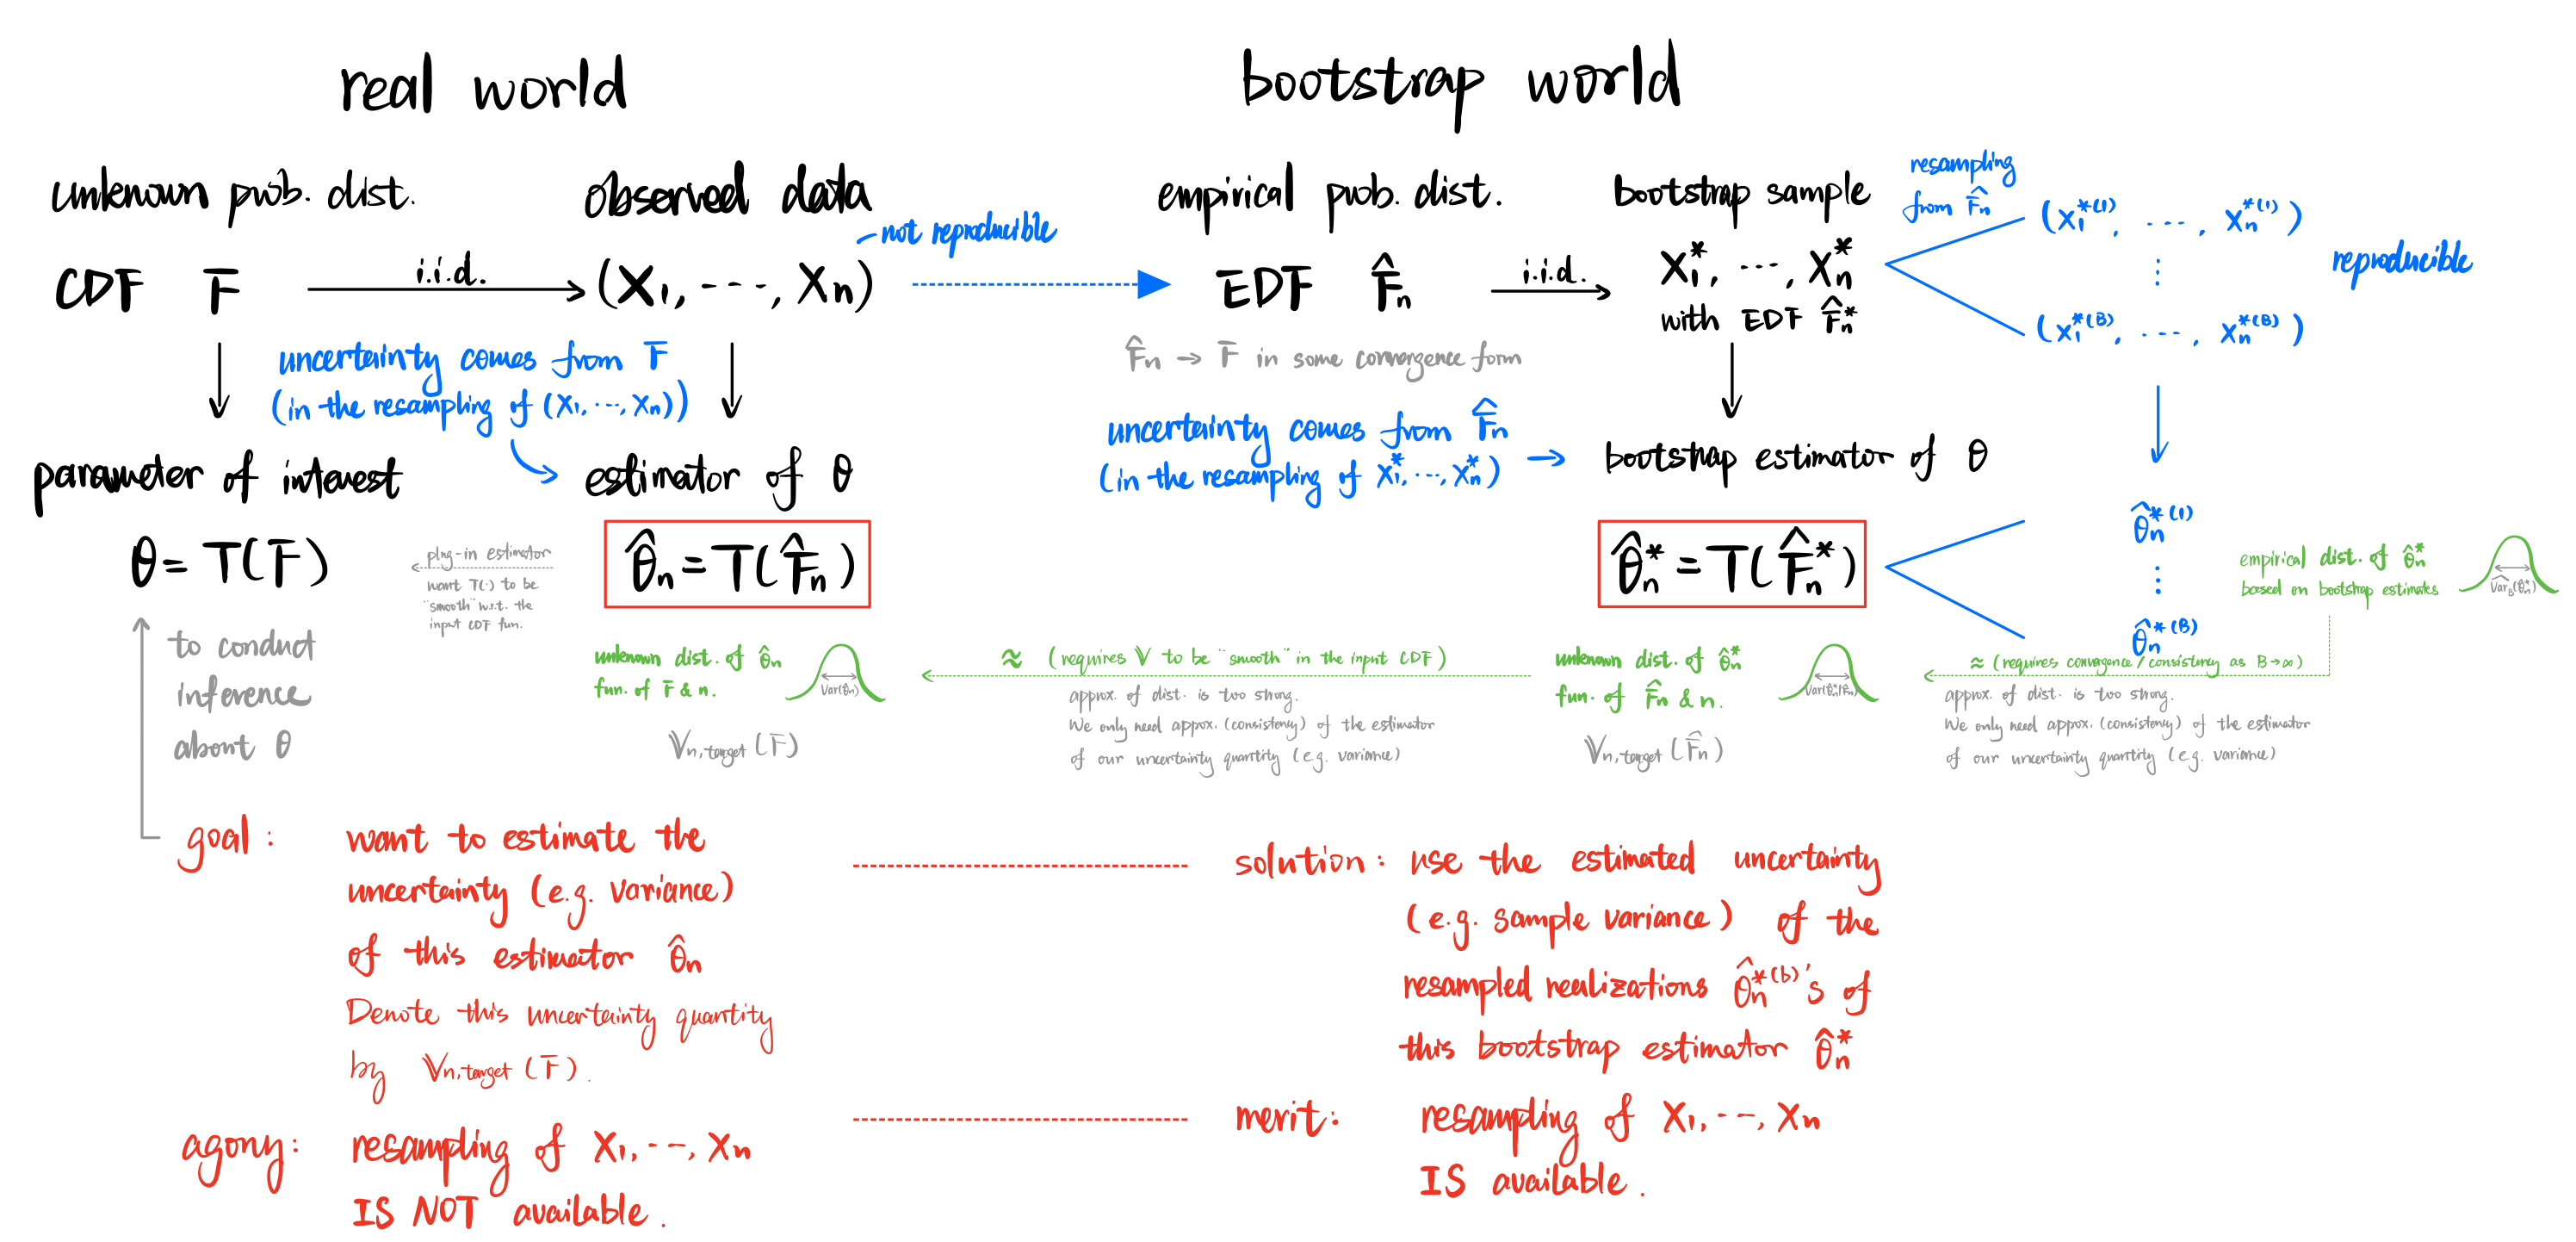
\includegraphics[width=0.9\linewidth]{figures/bootstrap-schematic.png}
    \caption{
    Think of bootstrap as an analogy of the real-world sampling process. Replace population parameters by sample estimates. \red{Give table of one-one correspondence between the real-world sampling process and the bootstrap world. target parameter  vs estimate, inaccessible resampled estimates vs bootstrap estimates, pop mean vs bootstrap mean, Var(estimator) vs Var(bootstrap estimates), etc.}
    }
    \label{fig:bootstrap-schematic}
\end{figure}

\subsubsection{Bootstrap bias estimation}
The main appeal of bootstrap is that it can estimate almost any distributional feature of $\hat\theta$.
\begin{itemize}
    \item We can use the bootstrap replicates of $\hat\theta$ to estimate its \underline{density function}, called \emph{bootstrap pictures}, by applying a density estimation technique (e.g., histogram or kernel density estimator).
    \item We can use bootstrap to estimate the \underline{bias} of $\hat\theta$. 
    \footnote{However, for bootstrap, bias correction is less stable than standard-error estimation because bias is generally harder to estimate accurately. See the BPD logistic-regression example.}
    
    Formally,
    \[
        \operatorname{bias}(\hat\theta)=\E_F(\hat\theta)-\theta,
    \]
    and the bootstrap bias estimate is
    \[
        \widehat{\operatorname{bias}}_{\mathrm{boot}}(\hat\theta)
        =
        \E_{F_n}(\hat\theta^*)-\hat\theta
        \approx
        \bar\theta^*-\hat\theta.
    \]
    The corresponding bias-corrected estimator is
    \[
        \hat\theta_{\mathrm{boot,BC}}
        =
        \hat\theta-\widehat{\operatorname{bias}}_{\mathrm{boot}}(\hat\theta)
        =
        2\hat\theta-\bar\theta^*.
    \]
\end{itemize}
 


\subsubsection{Bootstrap confidence intervals and tests}
\begin{enumerate}
    \item \textbf{Normal approximation interval.}
    Keep the usual normal form
    \[
        \hat\theta
        \pm
        z_{1-\alpha/2}\widehat{\mathrm{se}}_{\mathrm{boot}}(\hat\theta).
    \]
    This interval is the simplest to compute but reasonable only when the sampling distribution of $\hat\theta$ is close to normal.

    \item \textbf{Percentile interval.}
    Replace the normal approximation by quantiles of the ordered bootstrap replications
    \[
        \hat\theta_{(1)}^* \le \hat\theta_{(2)}^* \le \cdots \le \hat\theta_{(B)}^*.
    \]
    The nominal $100(1-\alpha)\%$ interval is
    \[
        \left(
            \hat\theta^*_{(\lfloor \alpha B/2\rfloor)},
            \hat\theta^*_{(\lfloor (1-\alpha/2)B\rfloor)}
        \right),
    \]
    with the obvious endpoint-index adjustment in actual computation if an index is $0$.

    \item \textbf{Basic, or type-2 percentile, interval.}
    Work with the \emph{bootstrap errors}
    \[
        \phi_b^*=\hat\theta_b^*-\hat\theta.
    \]
    After ordering $\phi_{(1)}^*\le\cdots\le\phi_{(B)}^*$, use
    \[
        \left(
            \hat\theta-\phi^*_{(\lfloor (1-\alpha/2)B\rfloor)},
            \hat\theta-\phi^*_{(\lfloor \alpha B/2\rfloor)}
        \right).
    \]
    The key idea is that the sampling \emph{error} is better approximated by the bootstrap than the parameter itself: we approximate $\hat\theta-\theta$ by the bootstrap error $\hat\theta^*-\hat\theta$, rather than using $\hat\theta^*$ directly as in the percentile method.
    
    \item \textbf{Bootstrap-$t$ interval.}
    Studentize each bootstrap replication:
    \[
        T_b^*
        =
        \frac{\hat\theta_b^*-\hat\theta}
             {\widehat{\mathrm{se}}(\hat\theta_b^*)}.
    \]
    If $T^*_{(1)}\le\cdots\le T^*_{(B)}$, use
    \[
        \left(
            \hat\theta-\widehat{\mathrm{se}}(\hat\theta)T^*_{(\lfloor (1-\alpha/2)B\rfloor)},
            \hat\theta-\widehat{\mathrm{se}}(\hat\theta)T^*_{(\lfloor \alpha B/2\rfloor)}
        \right).
    \]
    This requires a formula for $\text{se}(\hat\theta)$ (could be obtained from bootstrap, but we would need a nested bootstrap to estimate $\text{se}(\hat\theta_b^*)$). \footnote{Asymptotically, the bootstrap-$t$ method can have error $O_p(n^{-1})$ compared with $O_p(n^{-1/2})$ for the percentile method, but in finite samples it can be unstable if $\widehat{\mathrm{se}}(\hat\theta_b^*)$ is itself unstable.}
    \footnote{\textbf{Practical comparison.} The percentile interval is easy, stable, and range-preserving when the statistic's range matters, but its coverage can be poor. The bootstrap-$t$ interval has better asymptotic coverage when a good standard-error estimate is available, but it can be harder to compute, harder to explain, and unstable if the standard-error estimate is unstable.}

    \item \textbf{Bootstrap hypothesis test.}
    For a two-sample null hypothesis $H_0:F=G$, pool the two observed samples $X_1,\ldots,X_n \quad\text{and}\quad Y_1,\ldots,Y_m$ into one empirical sample of size $n+m$. Let $T(X,Y)$ be the observed two-sample test statistic computed from the original labeled groups. The achieved significance level is
    \[
        \operatorname{ASL}
        =
        \prob_{H_0}\{T(X^*,Y^*)\ge T(X,Y)\}.
    \]
    The bootstrap test approximates this null probability by repeatedly drawing $n+m$ observations with replacement from the pooled sample, assigning the first $n$ resampled observations to group 1 and the remaining $m$ to group 2, computing $T(X_b^*,Y_b^*)$, and using
    \[
        \widehat{\operatorname{ASL}}_{\mathrm{BOOT}}
        =
        \frac{\#\{b:T(X_b^*,Y_b^*)\ge T(X,Y)\}}{B}.
    \]
    This is close in spirit to a permutation test, except the bootstrap samples with replacement.
\end{enumerate}

\subsection{Cross-validation and prediction error}
\begin{itemize}
    \item Cross-validation targets \emph{prediction error} rather than the sampling distribution of an estimator. Its efficiency comes from using every observation for both training and validation, but never for both in the same fold.
    \item  In a regression problem, prediction error is $PE=\E\{(y-\hat y)^2\}$, where $(x,y)$ is a \emph{future (unseen)} observation. The residual squared error $RSE=\frac{1}{n}\sum_{i=1}^n (y_i-\hat y_i)^2=\frac{RSS}{n}$ is optimistic because the same data are used to fit and evaluate the model. \emph{Leave-one-out cross-validation (LOOCV)} corrects this by fitting without observation $i$ and evaluating at the omitted point:
    \[
        CV=\frac{1}{n}\sum_{i=1}^n (y_i-\hat y_i^{(-i)})^2.
    \]
    \item In $K$-fold cross-validation, split the data into $K$ roughly equal parts. For each fold $k$, fit the model on the other $K-1$ folds, evaluate prediction error on the held-out fold, and then average the $K$ held-out error estimates.
\end{itemize}


\begin{mybox}
\textbf{Analytical cross-validation errors for linear regression.}
\begin{enumerate}
    \item For ordinary least squares, write $\hat y=Hy$, where $H=X(X^\top X)^{-1}X^\top$ is the hat matrix.
    \item Use the leave-one-out identity
    \[
        y_i-\hat y_i^{(-i)}
        =
        \frac{y_i-\hat y_i}{1-h_{ii}},
    \]
    where $h_{ii}$ is the $i$th diagonal element of $H$. Therefore,
    \[
        CV
        =
        \frac{1}{n}
        \sum_{i=1}^n
        \left(
            \frac{y_i-\hat y_i}{1-h_{ii}}
        \right)^2.
    \]
    \item Replacing $h_{ii}$ by $\bar h=n^{-1}\sum_i h_{ii}$ gives \emph{generalized cross-validation} (GCV):
    \[
        GCV
        =
        \frac{RSS/n}{(1-\bar h)^2}.
    \]
    In OLS, $\sum_i h_{ii}=\tr(H)=p$, the number of fitted parameters / degrees of freedom of the fit.
\end{enumerate}
\end{mybox}

Even when analytical approximations such as LOOCV shortcuts, GCV, or prediction-error criteria are available, real cross-validation remains useful. These approximations rely on assumptions, and their degrees of freedom may be unclear for more adaptive procedures such as CART or nonparametric smoothing. By directly refitting the model on training folds and evaluating held-out observations, cross-validation gives a more robust empirical estimate of future prediction error.

\subsection{Model selection criteria}
\begin{itemize}
    \item Prediction-error criteria adjust goodness of fit by adding a penalty for model complexity. Common criteria include:
    \[
        C_p=\frac{RSS}{n}+\frac{2p\hat\sigma^2}{n},
        \qquad
        AIC=-2\log L(\hat\theta)+2p,
        \qquad
        BIC=-2\log L(\hat\theta)+\log(n)p,
    \]
    where $p$ is the number of fitted parameters. 
    \item BIC has the heavier penalty when $n$ is large and is \underline{consistent} for model selection (i.e., chooses the  correct model as $n\to \infty$) under the proper conditions.
\end{itemize}

\subsection{Bootstrap optimism correction for prediction error}
\red{This section needs further refinement. The interpretation does not seem correct. The key bias seems to be due to using the same samples in bs to train and evaluate the model RSE.}

The residual squared error is usually too small as an estimate of future prediction error because the same data are used to fit and evaluate the model. This downward bias is called \emph{optimism}: the amount by which apparent training error underestimates true prediction error.

For the $b$th bootstrap sample, fit the model and let $\hat\beta_b^*$ be the fitted coefficient vector. Compare two errors for this same fitted model:
\[
    \frac{1}{n}\sum_{i=1}^n
    \left(y_i-x_i'\hat\beta_b^*\right)^2
    \qquad\text{and}\qquad
    \frac{1}{n}\sum_{i=1}^n
    \left(y_i^*-{x_i^*}'\hat\beta_b^*\right)^2.
\]
The first evaluates the bootstrap-fitted model on the \emph{original} data, so it behaves more like \emph{test error}. The second evaluates it on the bootstrap sample used to \emph{fit} the model, so it is an optimistic \emph{training error}. Their difference estimates optimism for bootstrap sample $b$ (i.e., how much my training error underestimates the ``test error''):
\[
    \omega_b
    =
    \frac{1}{n}\sum_{i=1}^n
    \left(y_i-x_i'\hat\beta_b^*\right)^2
    -
    \frac{1}{n}\sum_{i=1}^n
    \left(y_i^*-{x_i^*}'\hat\beta_b^*\right)^2
    = 
    \text{``test error -- training error''}.
\]
Average these differences over bootstrap samples, $\hat\omega=\frac{1}{B}\sum_{b=1}^B\omega_b$, and estimate prediction error by
\[
    \frac{1}{n}\sum_{i=1}^n
    \left(y_i-x_i'\hat\beta^*\right)^2
    +
    \hat\omega,
\]
where $\hat\beta^* = \frac{1}{B} \sum_{b=1}^B \hat\beta_b^*$.

In short, the bootstrap estimates how overly optimistic the apparent error is, then adds that optimism back to get a better estimate of future prediction error.



\subsection{Bayesian computational addendum}
\subsubsection{Bayesian central limit theorem}
The Bayesian CLT is a large-sample normal approximation to a posterior distribution based on the posterior kernel 
\[
    p^*(\theta |  x)=p(x |  \theta)\pi(\theta).
\]
Let $\hat\theta_m$ be the posterior mode, solving $\frac{\partial}{\partial \theta_j}\log p^*(\theta |  x)=0,\ j=1,\ldots,p$.\\
Define the observed negative Hessian
\[
    H(\theta)
    =
    -
    \left[
        \frac{\partial^2 \log p^*(\theta |  x)}
             {\partial\theta_i\,\partial\theta_j}
    \right]_{i,j=1}^p.
\]

\textbf{Theorem 3.1 (Bayesian CLT).}\\
Suppose $x_1,\ldots,x_n \stackrel{i.i.d.}{\sim} p(x | \theta)$. The prior $\pi(\theta)$ may be improper, the posterior is proper, and the posterior mode exists, then as $n\to\infty$,
\[
    \theta |  x
    \stackrel{d}{\rightarrow}
    N_p\!\left(\hat\theta_m, H(\hat\theta_m)^{-1}\right).
\]
In other words, the posterior distribution converges to a normal distribution centered at the posterior mode.
\footnote{This is proved using Taylor expansion of $\log p^*(\theta | x)$ around $\hat\theta_m$: the first derivative term is zero at the mode, and the quadratic term gives a normal kernel.}

\begin{mybox}
\textbf{How to use the Bayesian CLT.}\footnote{See Examples 3.1--3.3.}
\begin{enumerate}
    \item Write the posterior kernel $p^*(\theta | x)=p(x | \theta)\pi(\theta)$.
    \item Find the posterior mode $\hat\theta_m$ by solving the score equations for $\log p^*(\theta | x)$.
    \item Compute $H(\hat\theta_m)$, the negative Hessian of the log posterior kernel at the mode.
    \item Approximate the posterior by $N_p(\hat\theta_m,H(\hat\theta_m)^{-1})$.
\end{enumerate}
\end{mybox}


\subsubsection{Gibbs sampling and MCMC}
MCMC is needed when noniterative methods such as importance sampling, rejection sampling, or weighted bootstrap are hard to tune in high-dimensional posterior problems. MCMC constructs a Markov chain from the \emph{univariate full conditional distributions} whose joint stationary distribution is the target posterior.

For $U=(U_1,\ldots,U_k)$ (whose joint distribution is the target), the Gibbs sampler assumes we \emph{can} sample (by any method) from the univariate full conditional distributions\footnote{In fact, we just need their kernels. If they do not belong to a known family, we can use rejection sampling, importance sampling, or a weighted bootstrap step inside Gibbs to get the needed draws.
}
\[
    p(u_i |  u_j,\ j\ne i),
    \qquad i=1,\ldots,k.
\]

\begin{mybox}
\textbf{Gibbs sampling algorithm.}
\begin{enumerate}
    \item Start from arbitrary initial values $(U_1^{(0)},\ldots,U_k^{(0)})$.
    \item At iteration $t+1$, Draw a sample for each coordinate sequentially:
    \[
        U_i^{(t+1)}
        \sim
        [U_i |
        U_1^{(t+1)},\ldots,U_{i-1}^{(t+1)},
        U_{i+1}^{(t)},\ldots,U_k^{(t)}],
    \]
    for $i=1,\ldots,k$. In many situations, we need to use a rejection algorithm to draw these samples.
    \item After enough iterations, use $(U_1^{(t)},\ldots,U_k^{(t)})$ as \emph{dependent} draws from the target joint distribution.
\end{enumerate}
\end{mybox}

(\textbf{Theorem 3.2.})
Under mild conditions, the Gibbs sampling distribution converges to the target distribution:
\[
    (U_1^{(t)},\ldots,U_k^{(t)})
    \stackrel{d}{\rightarrow} 
    [U_1,\ldots,U_k]
    \qquad \text{as } t\to\infty,
\]
and the convergence is exponential in $t$.
\footnote{distance between current sampler distribution and target distribution = $O(\rho^t)$, i.e., $\left\|\mathcal{L}\!\left(U^{(t)}\right)-\pi\right\|_{\mathrm{TV}} \leq C\rho^t, \ 0<\rho<1$, where $\mathcal L(U^{(t)})$ is the distribution of the Gibbs sampler after $t$ iterations, and $\|\cdot\|_{\mathrm{TV}}$ is total variation distance.} 
\footnote{A Rao-Blackwellized marginal posterior density estimate is given by
\[
    \hat p(u_i | x)= \frac{1}{m} \sum_{j=1}^m p(u_i | u_{-i, j}^{(t)}, x),
\]
where $m$ is the number of Gibbs sampler draws. This estimator has reduced variance compared to a kernel density estimate based only on sampled $u_i$ values.
}


\begin{mybox}
\textbf{Final comparison: jackknife, bootstrap, cross-validation, and MCMC.}
\begin{itemize}
    \item \underline{Jackknife:} targets bias reduction and variance estimation for smooth statistics by deleting one observation at a time; it can fail for nonsmooth statistics such as the sample median. (See Notes pp.~2--11.)
    \item \underline{Bootstrap:} targets standard errors, bias, sampling distributions, confidence intervals, and some tests by replacing $F$ with $F_n$ or $F_{\hat\eta}$; confidence intervals need many replications and careful calibration. (See Notes pp.~12--88, 109--111.)
    \item \underline{Cross-validation:} targets future prediction error and model selection by repeatedly fitting on training data and evaluating held-out observations; it is not estimating the sampling distribution of $\hat\theta$. (See Notes pp.~89--108.)
    \item \underline{MCMC / Gibbs:} targets posterior simulation when direct independent sampling is hard by constructing a convergent Markov chain; the draws are dependent and require convergence assessment. (See Gibbs notes pp.~370--378.)
\end{itemize}
\end{mybox}
